\cleardoublepage\chapter{Wireless Sensor Networks}\index{Wireless Sensor Network|textbf}\index{WSN|see{Wireless Sensor Network}}\label{chap:network}
\begin{figure}[tbhp]
 \centering
 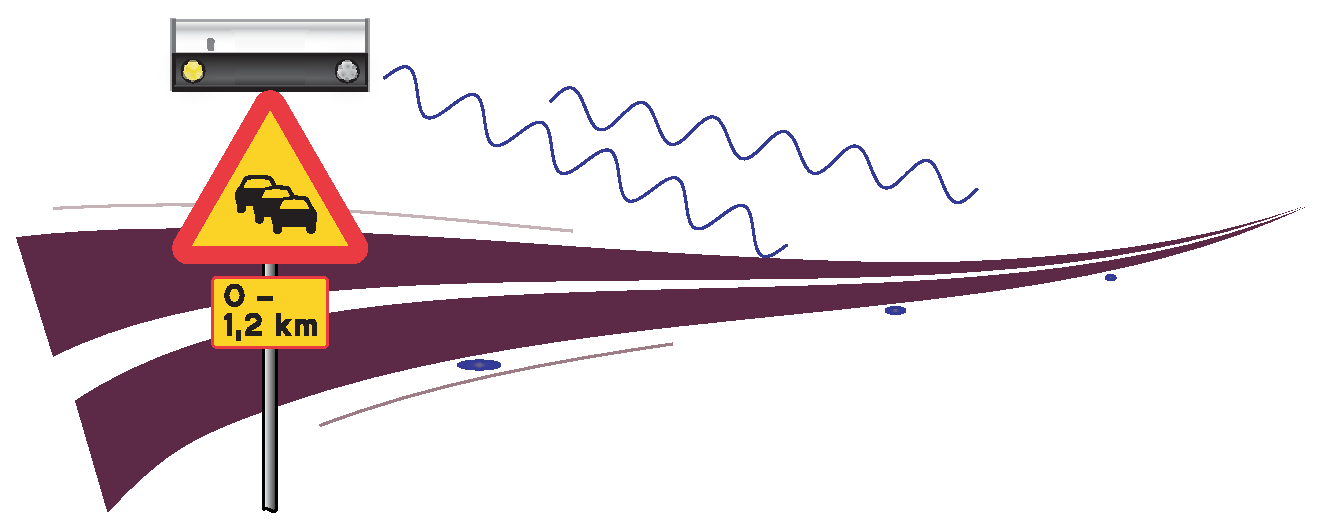
\includegraphics[width=1\linewidth]{images/queueRoad}
 % queueRoad.eps: 1179666x1179666 pixel, 300dpi, 9987.84x9987.84 cm, bb=
 \caption[Wireless Sensor Network]{Wireless Sensor Network together with a queue warning sign fitted with Amparo SeeMe\mtm\index{Amparo SeeMe}\index{SeeMe\mtm|see{Amparo SeeMe\mtm}} flashing unit.}
 \label{fig:queueRoad}
\end{figure}

\section[``Ambient Intelligence'' or putting electronics into groceries]{``Ambient Intelligence'' or\\ putting electronics into groceries}
\textsc{There has been} a tendency for some time now to put embedded computational power into large things such as washing machines and refrigerators. That tendency is not limited to large appliances but even disposable goods, groceries, living spaces and working spaces will soon be or already are endowed with such capabilities~\cite{Karl70}. Computational power that surrounds us in our daily lives can be -- somewhat praisefully -- called \mbox{``Ambient Intelligence''}\index{``Ambient Intelligence''} wherein many different devices will work together to control processes or interact with us. We should take this technology for granted, it should be unobtrusive and even invisible.

In the light of this, a new type of network emerged -- the Wireless Sensor Network\index{Wireless Sensor Network} (WSN). Each individual node in the network is capable of sensing or interacting with its environment. However, it is first when they are connected to each other that they show their true power. WSNs have many applications and the technical solutions are very different. 
 	
An interesting example of a WSN is the ``Smart Dust''\index{Smart Dust} proposed by the U.S.~Defence Advanced Projects Agency (DARPA). The smart-dust sensor nodes are extremely small - about the size of a grain of sand or even a dust-particle. The idea is to scatter thousands of these small sensors on the battlefield as an intelligent minefield to detect and monitor enemy movement.  The sensors can be spread out using aeroplanes or submunitions. An interesting civilian usage of these ``intelligent minefields''\index{intelligent minefields} can be found in accidents and catastrophe sites such as after an earthquake where humans can be trapped and wounded and need to be found quickly~\cite{runes}.

The usage for the WSN we are proposing is entirely related to traffic. One interesting application can be seen in Figure~\ref{fig:queueRoad} and is a queue warning system. The sensor nodes collaborate and send a signal to the warning unit if there is a queue.

\section{Wireless Hardware}

The transceiver could use IEEE 802.15.4 and ZigBee\footnote{ZigBee Alliance, \url{www.zigbee.org}}\index{ZigBee Alliance} standards~\cite{arrigault2007}. The exact design of the WSN is not decided upon, here ZigBee is used for simplicity.
The sensor nodes should be able to perform short-range communication in small networks for which ZigBee and Wireless Personal Area Networks (WPANs) are ideal. Unlike Wireless Local Area Network (WLANs), WPANs allow for small, power-efficient, inexpensive solutions for a wide range of devices since they do not involve any or very little infrastructure~\cite{802.15.4}.

\subsection{ZigBee Networks}\index{ZigBee Networks}

A Low-Rate Wireless Personal Area Network (LR-WPAN) is a simple, low-cost communication for applications where resources are limited~\cite{802.15.4}. An LR-WPAN offer easy installation, reliable communication, short-range operation, low cost and low power consumption. Two types of devices can exist in such a network; reduced-function devices\index{reduced-function device} (RFD) and full function-devices\index{full-function device} (FFD). A FFD can talk to everyone while an RFD can only talk to a FFD. ZigBee Alliance\index{ZigBee Alliance} defines the network\index{network layer}, security\index{application support sublayer} and application support layers (API) on top of the physical\index{physical layer} (PHY) and media access layer\index{media access layer} (MAC) defined by IEEE Standard 802.15.4~\cite{zigbee,802.15.4}\index{IEEE Standard!802.15.4}.

The network will consist mostly of sensor nodes (SNs) which are RFDs. These can unlike the FFDs, not become the coordinator in the star topology\index{network topology!star topology} net used in this implementation~\cite{zigbee, 802.15.4}. We will use an access point (AP) to transmit data to the backbone network. The network topology can be seen in Figure \ref{fig:network}. In the future, we will like to have the option to use a mesh network topology\index{network topology!mesh topology} instead. This will allow us to use SNs as relays.

\begin{figure}[hbtp]
 \centering
 \begin{minipage}{1\linewidth}
  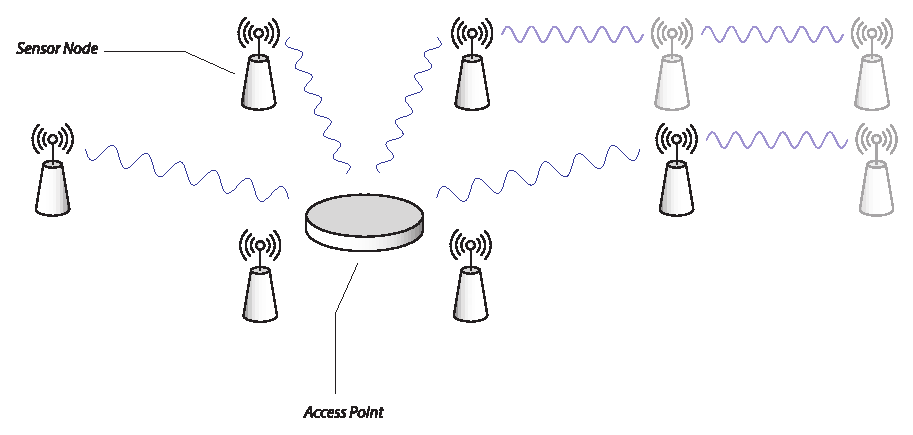
\includegraphics[width=1\linewidth]{images/network.eps}
 % network.eps: 1179666x1179666 pixel, 300dpi, 9987.84x9987.84 cm, bb=
 \caption[Mesh network topology]{Star network topology\index{network topology!star topology} with network coordinator~\cite{802.15.4, zigbee}. The network coordinator is in our application the access point (AP) and the nodes are the wireless sensor nodes (SNs).}
 \label{fig:network}
 \end{minipage}
\end{figure}
 	
\section[Wireless Sensor Networks for applications related to traffic]{Wireless Sensor Networks\\for applications related to traffic}
Due to the different applications, the requirements for a WSN are also different. In our application some of the important requirements are
\begin{itemize}
 \item \textbf{Multihop (wireless) communication\index{multihop communication}.} Sending information over large distances is only possible using high transmission power. By using sensor nodes as relays we can reduce the required power.
 
 \item \textbf{Energy-efficient operation\index{energy-efficient operation}.} Since the nodes are battery powered a strict power consumption policy is needed. When parts of the sensor node are not needed they are put to sleep only to be awaken when they are needed.
 
\item \textbf{Auto-configuration.\index{auto-configuration}} The nodes should be easily installed, by anyone, anywhere and at any time. If the sensor nodes, and the wireless network, can be auto-configured it would be hugely beneficial. A \mbox{``must-have''} property~\cite{rydstrom2006} of the sensor nodes is that they should autonomously position themselves in the network. Preferably they should not rely on surrounding infrastructure such as the Global Positioning System (GPS). There are many different techniques that forms the basis for autonomous positioning. %Time-of-flight, ToF, techniques has received attention lately.

\item \textbf{In-network processing.}\index{in-network processing} An individual node may not be able to determine whether an event has occurred or not but will depend on collaboration with its neighbours. We would like to keep the inter-node traffic as low as possible to keep the power consumption low at the same time as any calculations will take time, memory and power.
\end{itemize}

The amount of processing needed in the SNs is highly dependant on their use. There are three main usages for our equipment
\begin{itemize}
 \item \textbf{Vehicle detection\index{detection}, speed estimation\index{speed estimation} and counting,}
 \item \textbf{Vehicle classification\index{classification},}
 \item \textbf{Queue detection\index{queue detection}. See Figure~\ref{fig:queueRoad}.}
\end{itemize}

There is also a possibility to re-identify\index{re-identification} vehicles~\cite{cheung2005-1}. This requires more SNs and more computational power.